% TO-DO:
% * 

\documentclass[16pt]{beamer}

\ifdefined\chinchin
\usepackage[CJKspace]{xeCJK}
%\setCJKmainfont[BoldFont=SimHei,ItalicFont=AR PL KaitiM GB]{Alibaba PuHuiTi}
\setCJKmainfont{Alibaba PuHuiTi}
\newcommand{\cc}[2]{#1}
\else
\newcommand{\cc}[2]{#2}
\fi

%\usepackage{newtxtext,newtxmath}	% use Times Roman font
%\usepackage{newtxtext}
%\renewcommand{\familydefault}{\sfdefault}
%\usefonttheme{serif}
\usefonttheme{professionalfonts}
%\setbeamertemplate{theorems}[numbered]
\setbeamertemplate{caption}{\insertcaption} 	% no `Figure' prefix before caption

\mode<presentation> {

%\usetheme{default}
%\usetheme{AnnArbor}
%\usetheme{Antibes}
%\usetheme{Bergen}
%\usetheme{Berkeley}
%\usetheme{Berlin}
%\usetheme{Boadilla}
%\usetheme{CambridgeUS}
%\usetheme{Copenhagen}
%\usetheme{Darmstadt}
%\usetheme{Dresden}
%\usetheme{Frankfurt}
%\usetheme{Goettingen}
%\usetheme{Hannover}
%\usetheme{Ilmenau}
%\usetheme{JuanLesPins}
%\usetheme{Luebeck}
\usetheme{Madrid}
%\usetheme{Malmoe}
%\usetheme{Marburg}
%\usetheme{Montpellier}
%\usetheme{PaloAlto}
%\usetheme{Pittsburgh}
%\usetheme{Rochester}
%\usetheme{Singapore}
%\usetheme{Szeged}
%\usetheme{Warsaw}

%\usecolortheme{albatross}
%\usecolortheme{beaver}
%\usecolortheme{beetle}
%\usecolortheme{crane}
%\usecolortheme{dolphin}
%\usecolortheme{dove}
%\usecolortheme{fly}
%\usecolortheme{lily}
\usecolortheme{orchid}
%\usecolortheme{rose}
%\usecolortheme{seagull}
%\usecolortheme{seahorse}
%\usecolortheme{whale}
%\usecolortheme{wolverine}		% Hofstra

%\setbeamertemplate{footline} % To remove the footer line in all slides uncomment this line
\setbeamertemplate{footline}[page number] % To replace the footer line in all slides with a simple slide count uncomment this line
\setbeamertemplate{navigation symbols}{} % To remove the navigation symbols from the bottom of all slides uncomment this line
}

\setbeamertemplate{headline}{}
\setbeamersize{text margin left=1mm,text margin right=1mm} 
\settowidth{\leftmargini}{\usebeamertemplate{itemize item}}
\addtolength{\leftmargini}{\labelsep}

\usepackage[backend=biber,style=numeric]{biblatex}
\bibliography{../AGI-book}
\renewcommand*{\bibfont}{\footnotesize}
\setbeamertemplate{bibliography item}[text]

\usepackage{graphicx} % Allows including images
\usepackage{tikz-cd}
\usepackage[export]{adjustbox}% http://ctan.org/pkg/adjustbox
\usepackage{verbatim} % comments
% \usepackage{tikz-cd}  % commutative diagrams
% \newcommand{\tikzmark}[1]{\tikz[overlay,remember picture] \node (#1) {};}
% \usepackage{booktabs} % Allows the use of \toprule, \midrule and \bottomrule in tables
% \usepackage{amssymb}  % \leftrightharpoons
% \usepackage{wasysym} % frownie face
% \usepackage{newtxtext,newtxmath}	% Times New Roman font
% \usepackage{sansmath}

\newcommand{\emp}[1]{{\color{violet}#1}}
\newcommand{\vect}[1]{\boldsymbol{#1}}
\newcommand{\tab}{\hspace*{1cm}}
\newcommand*\confoundFace{$\vcenter{\hbox{\includegraphics[scale=0.2]{../confounded-face.jpg}}}$}
\newcommand{\smiley}{$\vcenter{\hbox{\includegraphics[scale=0.05]{../smiling-face.png}}}$}

%%%%%%%% Make table of contents %%%%%%%

\makeatletter
\renewcommand{\boxed}[1]{\fbox{\m@th$\displaystyle\scalebox{0.9}{#1}$} \,}
\makeatother
\newif\ifframeinlbf
\frameinlbftrue
\makeatletter
\newcommand\listofframes{\@starttoc{lbf}}
\makeatother
\addtobeamertemplate{frametitle}{}{%
	\ifframeinlbf
	\addcontentsline{lbf}{section}{\protect\makebox[2em][l]{%
			\protect\usebeamercolor[fg]{structure}\insertframenumber\hfill}%
		\insertframetitle\par}%
	\else\fi
}

%----------------------------------------------------------------------------------------
%	TITLE PAGE
%----------------------------------------------------------------------------------------

\title[Structure of logic once more]{\cc{再谈一次 AI 的逻辑结构}
{\Huge《AI and the structure of logic, once more》}}
\author{\cc{YKY 甄景贤}{YKY}} % Your name
%\institute[] % Your institution as it will appear on the bottom of every slide, may be shorthand to save space
%{
%Independent researcher, Hong Kong \\ % Your institution for the title page
%\medskip
%\textit{generic.intelligence@gmail.com} % Your email address
%}
\date{\today} % Date, can be changed to a custom date

\begin{document}

\frameinlbffalse
\addtocounter{page}{-1}
\begin{frame}[plain,noframenumbering]
\titlepage
\end{frame}

\addtocounter{page}{-1}
\begin{frame}[noframenumbering]
\frametitle{Table of contents}
\listofframes
\vspace*{0.5cm}
多谢 支持 \smiley
\end{frame}

%----------------------------------------------------------------------------------------
%	PRESENTATION SLIDES
%----------------------------------------------------------------------------------------

%------------------------------------------------

\frameinlbftrue

%\begin{frame}
%\frametitle{Fourier 神经网络}
%\begin{itemize}
%	\item 之前说过,需要 symmetric 神经网络。 可以用 \emp{多项式} 激活函数,得出一大堆 多项式的 weight-sharing 条件。 这方法在 层数 增大时,计算变得很复杂。 这是一个 computational invariant theory 的问题,我暂时未有时间深入研究
%	
%	\item 另一个方法我称之为 Fourier 神经网络
%	\item 命题空间 $\mathbb{P}\mathrm{rop}$
%\end{itemize}
%\end{frame}

\begin{frame}
\frametitle{「神经」知识表示}
为什么要研究 神经知识表示?
\begin{itemize}
	\item 从经典 logic-based AI 的传统,一直在使用「符号」的知识表示法

	\item 符号逻辑 很容易转换成 抽象代数/范畴论 形式(它们是同一个大家庭的「近亲」)
	
	\item 然而 或许存在 截然不同 的知识表示法? 但我们很难想像它 \emp{长什么样子}

	\item 人脑的「神经」知识表示,可以作为参考,然后再研究它和逻辑表示之间的 correspondence
\end{itemize}

\vspace*{0.4cm} 神经知识表示 的特点:
\begin{itemize}
	\item distributive(分布性)

	\item model-based (vs rule-based)

	\item \textit{in situ}(固定性)--- 例如辨认「猫」的时候,大脑中 相应的神经元被 激活,但这些 神经元 \emp{不能移动},所以「猫」的表示 也不可移动
\end{itemize}
问题是: 如果要辨认「白猫追黑猫」,「猫」的表示是固定的,则这两个「猫」表示 如何\emp{共存}於神经网络中?\\
答案很可能是: 两个「猫」\emp{交替}地 出现在 \emp{时间}上
\end{frame}

\begin{frame}
\frametitle{神经 特征簇 (feature clusters)}
例如,以「匙羹在杯中」作例子:
\begin{equation}
	\vcenter{\hbox{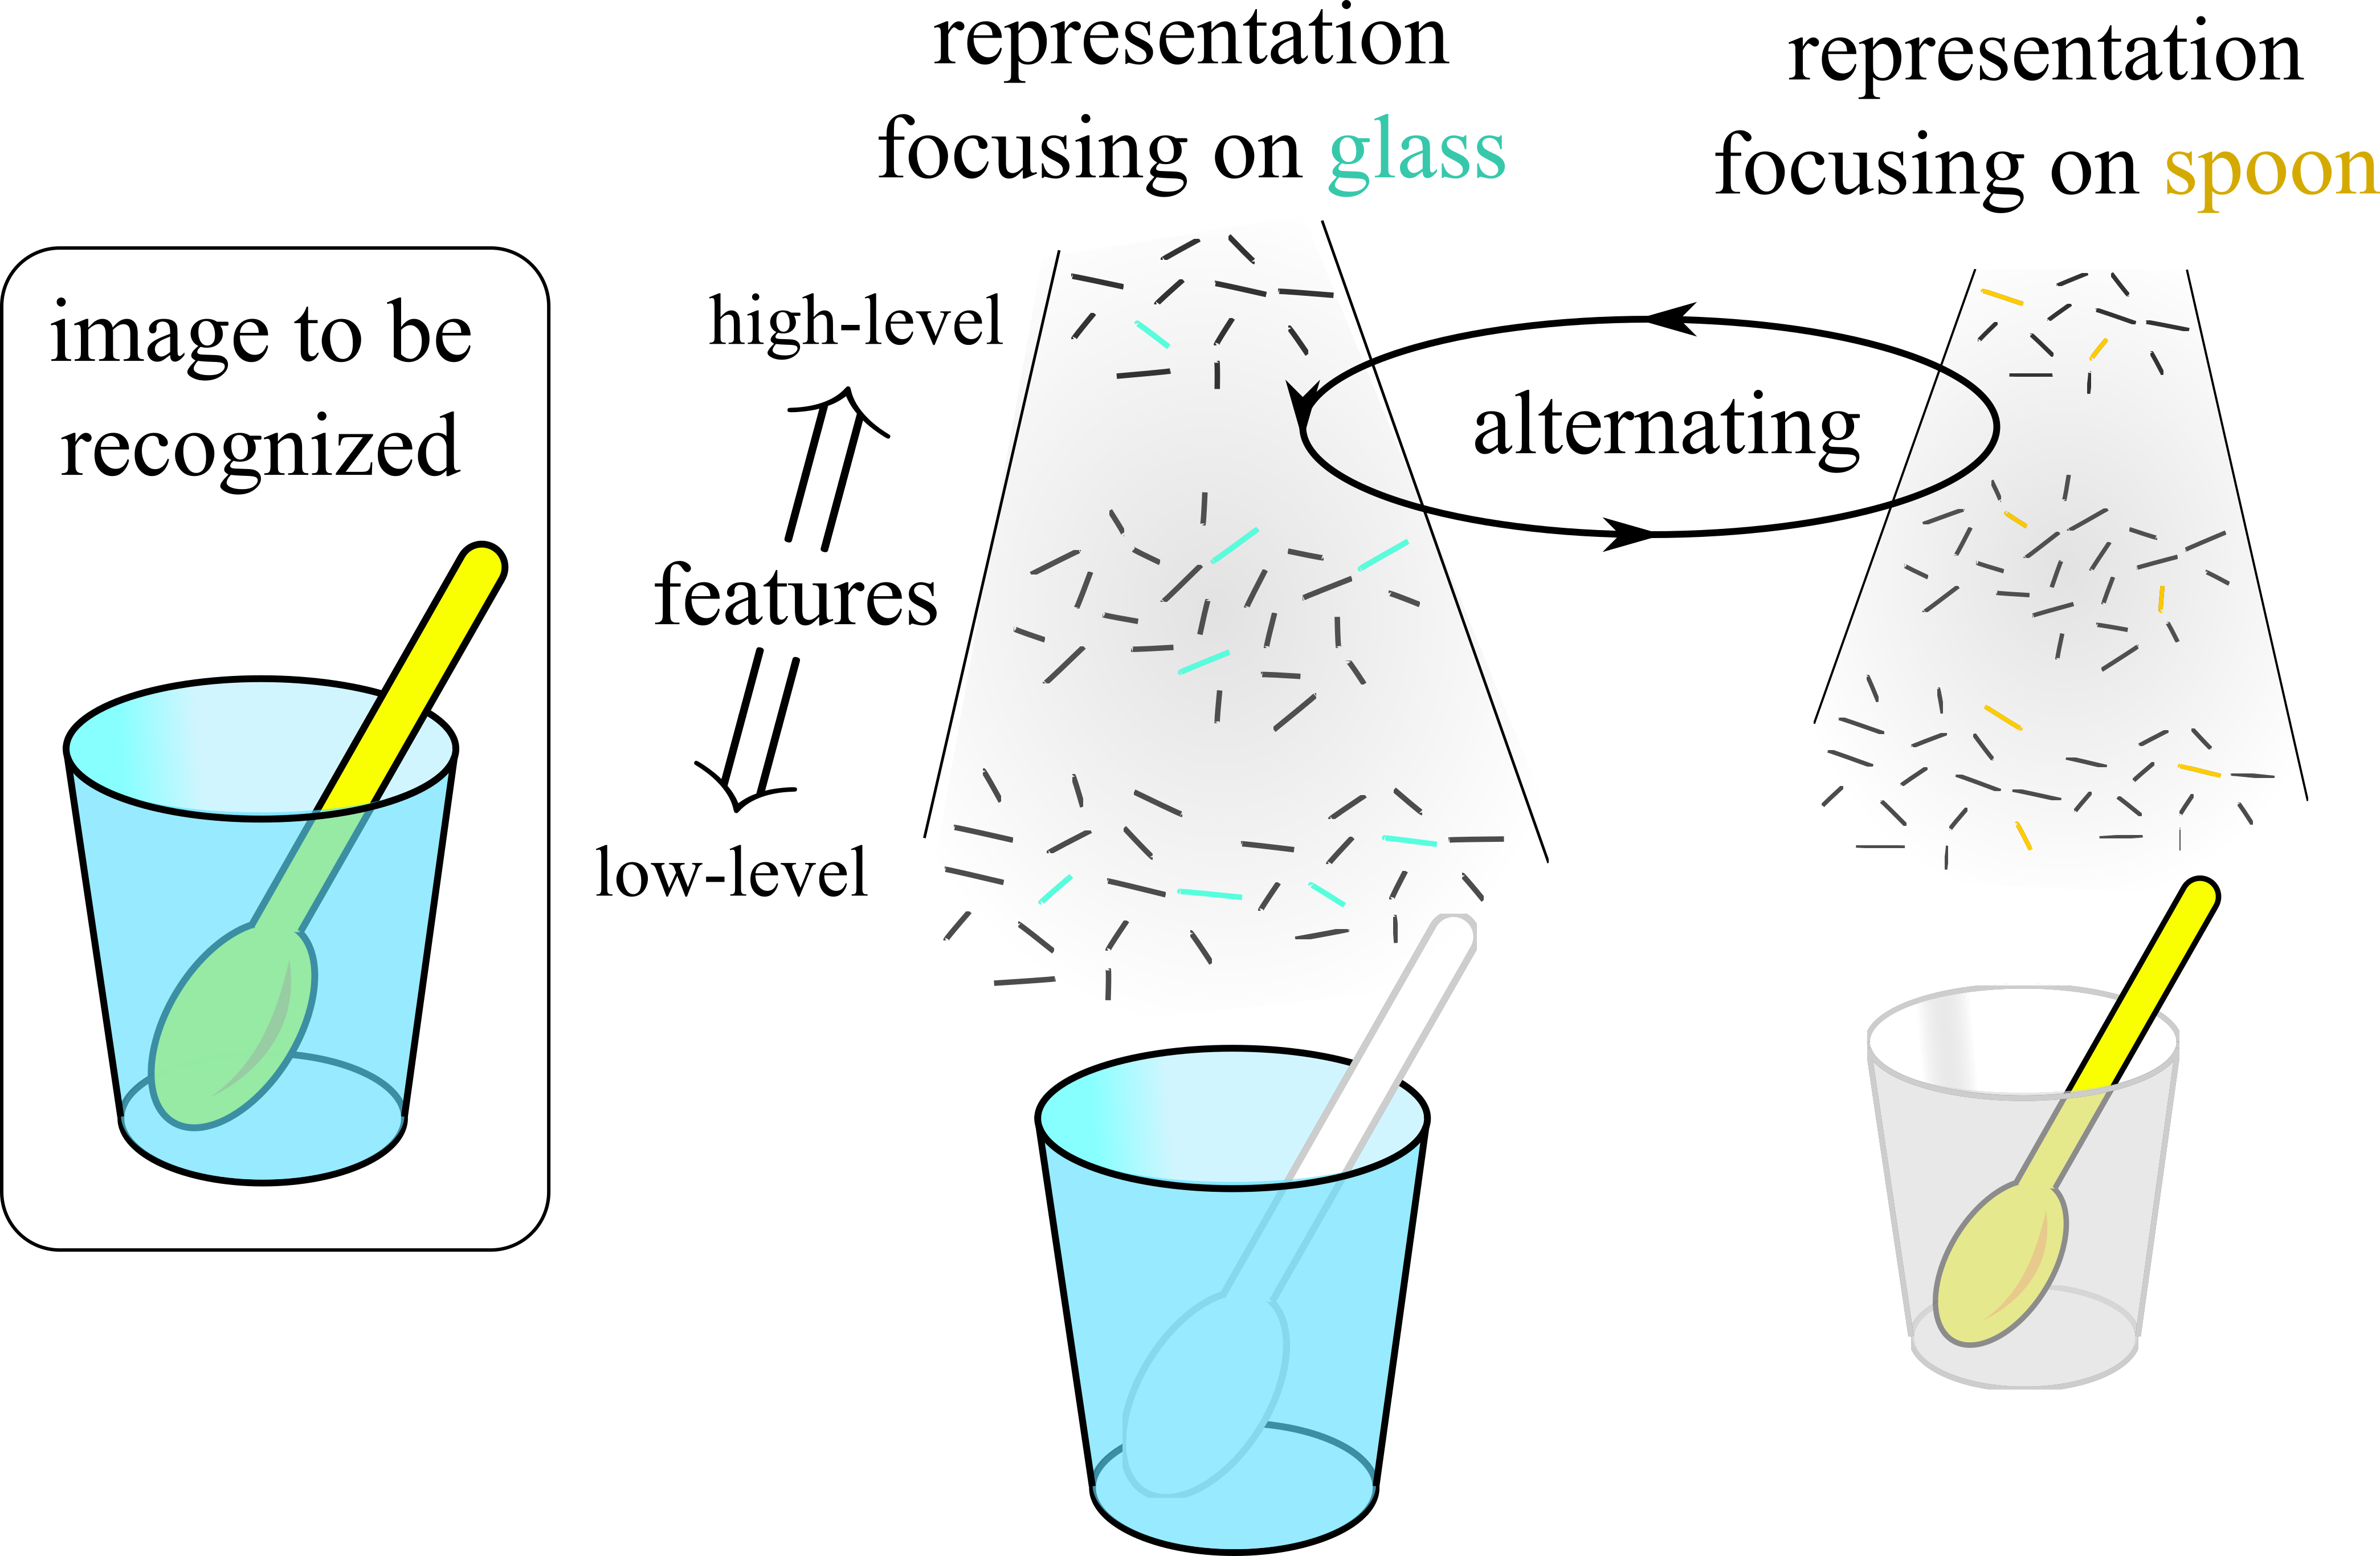
\includegraphics[scale=0.5]{neural-representation-alternating-glass-spoon.png}}}
\end{equation}
每个 复杂物体 由一个 \emp{feature cluster} 辨认。 多个「特征簇」在时间上交替出现,可以看成是一种 composition,例如 $A \cdot B$ 或 $A \circ B$.
\end{frame}

\begin{frame}
\frametitle{高阶 特徵}
\begin{itemize}
	\item 一串 特征簇 的时间序列,例如 $A \cdot B$,可以被 更\emp{高阶} 的神经网络 用作输入。 高阶辨认 的结果是一些关系 (relations),例如「匙羹\emp{在}杯\emp{内}」
	\begin{equation}
		\vcenter{\hbox{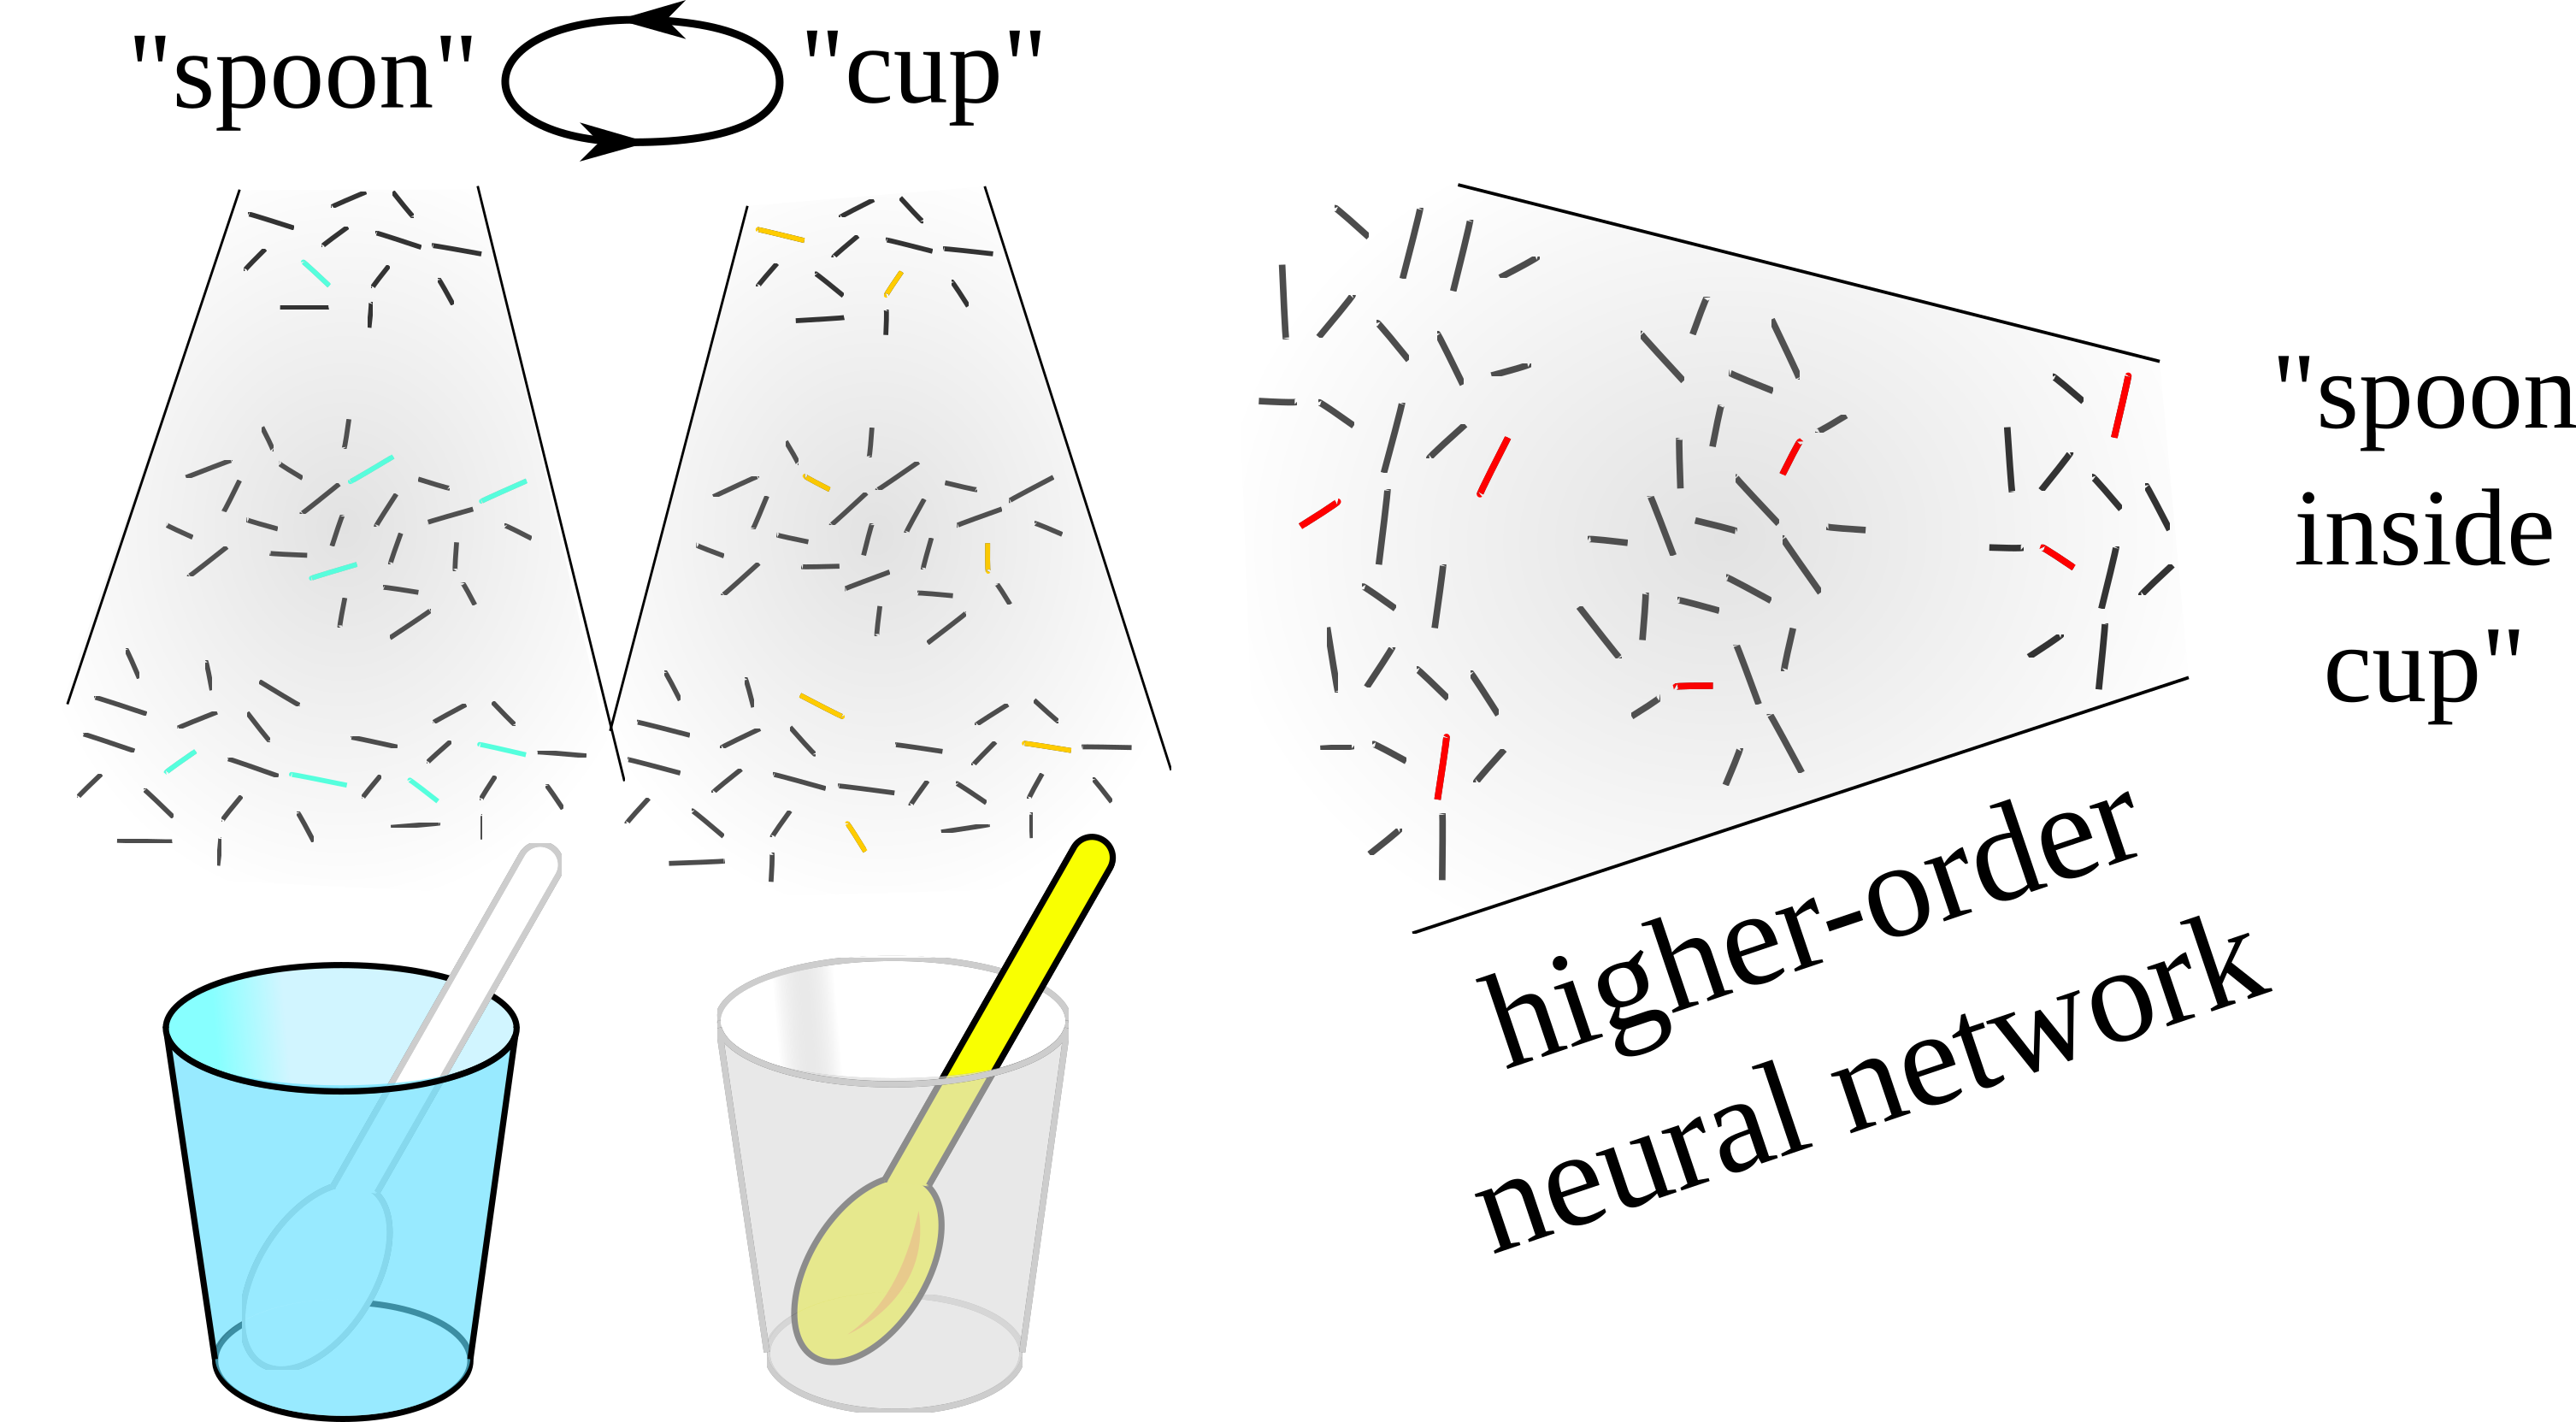
\includegraphics[scale=0.5]{higher-order-NN.png}}}
	\end{equation}
	
	\item 这似乎是一个 $\mbox{特征空间} \times \mbox{时间}$ 的映射 $f: X \times T \rightarrow Y$
	
	\item {\color{red}关於这部分其实我仍未肯定,或许有其他方法}
\end{itemize}
\end{frame}

\begin{frame}
\frametitle{关於 ``model-based reasoning'' 的质疑}
\begin{itemize}
	\item 很多人认为大脑的思考方式是 先在脑中构造 models,然后再从 models 中「读出」一些结论
	\item 例如给定一个描述:「已婚妇人出轨,用刀刺死丈夫」
	\begin{equation}
	\vcenter{\hbox{
\includegraphics[scale=0.7]{murder-scene.png}}}
	\end{equation}
	\item 如果假设「妻子有长头发」、「丈夫死时穿著西装」,这些都是 \emp{臆想} 出来的细节,是不正确的
	\item 那么这 model 可以有哪些细节? 答案是: 任何细节都不可以有,除非是 逻辑上蕴含的
	\item 例如我们可以假设妻子 probably 有一双手臂,但也有例外的情况是独臂的,这是一种 逻辑推导
	\item 所以,其实所谓 ``model-based reasoning'' 并没有那么神奇,也并不一定正确,它的细节必需被 \emp{逻辑} 约束
	\item 而 model 本身也可以用一些 抽象的逻辑命题 构成,这也是合理的; 反而,一个有很多感官细节的 model 并不合理
\end{itemize}
\end{frame}

\begin{frame}
\frametitle{神经 $\leftrightarrow$ 逻辑 correspondence}
\begin{itemize}
	\item 我们的目标是了解 神经表示 和 逻辑表示 之间的关系,这关系或许可以用范畴论描述?
	
	\item 定义 复杂情境 (complex scenario) 是 感知材料 (sensory data) 的一个片段,如:
	\begin{equation}
		\vcenter{\hbox{
\includegraphics[scale=0.5]{sensory-movie.png}}}
	\end{equation}
	又或者一个故事,例如「John 爱 Mary 但 Mary 不爱他」
	
	\item 一个复杂情境 可以用若干个 特征簇 描述
	
	\item Equivalently, 复杂情境 可以用 \emp{逻辑} 表示,就是一大堆 逻辑命题 的 conjunction,这些命题 钜细无遗 地描述该情境
\end{itemize}
\end{frame}

\begin{frame}
\frametitle{再谈一次 逻辑结构}
\begin{itemize}
	\item 以前曾经说过,机器视觉 的成功,有赖於 将 视觉的几何结构 impose 在深度神经网络上
	\item 这 深度神经网络 原本是 ``free'' 的,但加了限制之后,权重空间 变小了(例如维数降低),所以学习加速了
	\item 所谓 symmetry 的意义,简单例子:「如果知道左边等於右边,那就只需计算一次」
	\item 换句话说,数学家喜欢对称性,是因为它经常可以简化计算
	\item 同理,我们想将 逻辑结构 的对称性 impose 到神经网络
	\item 实际上,可能只需要逻辑上的交换律,就可以达到 强人工智能,正如 机器视觉的成功,在於引入了 CNN 的 convolution 结构,后者只是 视觉不变性 的其中一个最显著的 invariant
	\item 现代逻辑理论 非常漂亮,我花了十多年时间才弄懂,我希望将这套 逻辑-学习 理论简单讲解一下,也算功德完满了
\end{itemize}
\end{frame}

\begin{frame}[plain]
\begin{itemize}
	\item 在经典时代,逻辑的 代数形式 可以用 Boolean algebra 表述,然而这方法只适用於 命题逻辑
	\item Boolean algebra 是中学生熟悉的,类似 Venn diagram 的结构
	\item 这种结构和 拓樸学 的 open sets 结构一样,所以 命题逻辑 也可以看成是一种 topology
	\item 然而 predicate logic 的结构更复杂,直到最近才有比较完善的表述
	\item 现代逻辑结构和 type theory 有深刻的关系,此即 Curry-Howard isomorphism
	\item 现代逻辑也涉及 topos theory,那是一种由 algebraic geometry 引入的结构
\end{itemize}
\end{frame}

\begin{frame}
\frametitle{Type theory and the Curry-Howard isomorphism}
\begin{itemize}
	\item 大家都知道 Lisp 语言没有 type,它是一种 untyped $\lambda$-calculus
	\item 在 Lisp 之上引入 type system,衍生成 ML, Caml, OCaml, Haskell 等 一系列语言
	\item 每一个 program 属於某个 type,例如 $\mathrm{length}()$ 函数,输入一个字串,输出它的长度; $\mathrm{length} : \mathsf{String} \rightarrow \mathsf{Integer}$
	\item 有些逻辑学家 察觉到 类型论 的 $\tau_1 \rightarrow \tau_2$ 和逻辑中 $P \rightarrow Q$ 是一模一样的
	\item 这个关系的发现者至少包括:  Brouwer-Heyting-Kolmogorov-Curry-\mbox{de Bruijn}-Howard
	\item 这关系的深刻之处,在於把 符号逻辑上的 proofs 和 程式语言 的 programs 划上等号,前者是 符号/静态的,后者是 程序/动态的
	\item 每个 proof 就是一个 program,它输入一些 arguments,输出 关於那些 arguments 的证明
	\item 例如: 「所有人都会死」是一个 program,它输入「苏格拉底」,输出「苏格拉底会死」 
	\item 这个对应也許可以应用到深度学习: 神经网络 也是一種 函數 / mapping,它将 逻辑前提 map 到结论
\end{itemize}
\end{frame}

\begin{frame}
\frametitle{Topos theory and fibrations}
\begin{itemize}
	\item Predicate logic (谓词逻辑)和 命题逻辑 之间的差异在於 fibration 结构
	\item Fibration 通常用 $\mathrel{\substack{\mathbb{E}\\\downarrow \\\mathbb{B}}  {\scriptstyle p}}$ 表示,$\mathbb{B}$ = base space, $\mathbb{E}$ = \`{e}tal\`{e} space, $p$ = projection
	\item Base space 是 type 的空间,\`{e}tale space 是 predicate 的空间
	\item 由於 Curry-Howard 对应, type = propositions,在 base 空间上只有 命题逻辑
	\item 例如 $\mathbb{B}$ 空间的一个 type 是 $\mathrm{Human}$,$\mathbb{E}$ 空间的一个谓词是 $\mathrm{Mortal}$
	\item 於是有以下这个 type inference rule:
	\begin{equation}
	i:\mathrm{Human} \vdash \mathrm{Mortal}(i): \mathsf{Prop}
	\end{equation}
	意思是说,如果 $i$ 属於 $\mathrm{Human}$ 类型,则 $\mathrm{Mortal}(i)$ 属於 $\mathsf{Prop}$ 类型
\end{itemize}
\end{frame}

\begin{frame}[plain,allowframebreaks]
\begin{itemize}
	\item $H(a)$ is a type.
	\item $H$ is a prodicate type.
	\item The proof of $H(a)$ may be the tuple $(a, H)$ or $a \in H$
\end{itemize}
\end{frame}

\frame[allowframebreaks]{
\cc{多谢收看}{Thanks for watching} \smiley
% \frametitle{References}
\printbibliography
}

\end{document} 